 \documentclass[a4paper]{article}

%NOTE BY DIRK: 	Gelieve paragrafen gewoon in te typen, geen \par gedoe.
%								Citaties liefst in de vorm "author:1999" met author=achternaam van de eerste auteur
%								figuren, tabellen, listings, ... met prefixen: fig, tab, lst, ...


\author{Olivier Berghmans, Nick De Frangh, Dirk Delahaye,\\Kristof Overdulve, Pieter-Jan Pintens, Tobias Van Bladel}
\title{Architectuur en Algoritmen van Computer Games\\\textbf{Hovercraft Universe}\\\small{\url{http://uhasseltaacgua.googlecode.com/}}}
\pagestyle{plain}
\usepackage[dutch]{babel}
\usepackage{amsfonts}
\usepackage{graphicx}
\usepackage{url}
\usepackage{todonotes}
\usepackage{hyperref}
\usepackage{parskip}
\usepackage{listings}
\hypersetup{
%    bookmarks=true,         % show bookmarks bar?
    unicode=false,          % non-Latin characters in Acrobat�s bookmarks
    pdftoolbar=true,        % show Acrobat�s toolbar?
    pdfmenubar=true,        % show Acrobat�s menu?
    pdffitwindow=false,     % window fit to page when opened
    pdfstartview={FitH},    % fits the width of the page to the window
    pdftitle={Architectuur en Algoritmen van Computer Games},    % title
    pdfauthor={Olivier Berghmans, Nick De Frangh, Dirk Delahaye, Kristof Overdulve, Pieter-Jan Pintens, Tobias Van Bladel},     % author
    pdfsubject={Hovercraft Universe},   % subject of the document
    %pdfcreator={Creator},   % creator of the document
    %pdfproducer={Producer}, % producer of the document
    %pdfkeywords={keywords}, % list of keywords
    pdfnewwindow=true,      % links in new window
    colorlinks=true,       % false: boxed links; true: colored links
    linkcolor=black,          % color of internal links
    citecolor=green,        % color of links to bibliography
    filecolor=magenta,      % color of file links
    urlcolor=cyan           % color of external links
}

\begin{document}

\maketitle

\tableofcontents
\newpage

\section{Introductie}
\emph{Hovercraft Universe} is een race game waarin spelers tussen planeten in de ruimte kunnen rondvliegen met hovercrafts. Het nadeel aan traditionele race games is dat de camera en game play nogal statisch en weinig beweeglijk is. Dit spel is revolutionair in het opzicht dat wanneer je van planeet naar planeet springt de speler in een andere atmosfeer komt met een ander niveau van zwaartekracht en andere eigenschappen.

\section{Gebruikte libraries}
%MAXIMUM 2 ZINNEN PER ENTRY!!!
\begin{itemize}
\item[\textbf{Physics}] De fysische gamewereld wordt gesimuleerd door Havok Physics\footnote{\url{http://www.havok.com/index.php?page=havok-physics}}. Havok draait enkel op de server en zorgt voor alle berekeningen die nodig zijn voor fysische interactie.

\item[\textbf{Rendering}] Voor het renderen gebruiken we de Ogre Open Source Graphics Engine\footnote{\url{http://www.ogre3d.org/}}. Ogre draait enkel op de clients en zorgt voor de visuele representatie van de game-entiteiten. Andere, uitsluitend visuele, effecten en overlays worden ook door Ogre afgehandeld: particle effects, tekst overlays boven de entiteiten, \ldots. SkyX\footnote{\url{http://www.ogre3d.org/forums/viewtopic.php?t=48414&f=11}} en OgreMax\footnote{\url{http://www.ogremax.com/}}.

\item[\textbf{Netwerk}] ZoidCom\footnote{\url{http://www.zoidcom.com/}}

\item[\textbf{Input}] Object Oriented Input System (OIS)\footnote{\url{http://sourceforge.net/projects/wgois/}}

\item[\textbf{Geluid}] FMOD Interactive Audio Middelware\footnote{\url{http://www.fmod.org/}}

\item[\textbf{Scripting}] Lua\footnote{\url{http://www.lua.org/}} en LuaBind\footnote{\url{http://www.rasterbar.com/products/luabind.html}} bieden de mogelijkheid om op een dynamische manier eigenschappen van het spel te veranderen.

\item[\textbf{GUI}] Adobe Flash\footnote{\url{http://www.adobe.com/products/flash/}} en Hikari\footnote{\url{http://code.google.com/p/hikari-library/}}.

\end{itemize}

\section{Programmastructuur en -organisatie}
\subsection{Algemeen}
De basisstructuur van de engine achter Hovercraft Universe is gemaakt naar analogie met de architectuur van \emph{Shellshock: Nam '67} \cite{rouwe:2005}. Elk object in de spelwereld waarmee ge\"interageerd kan worden, wordt voorgesteld door een \texttt{Entity}. Deze entiteiten worden gegroepeerd in de \texttt{EntityManager}, die de entiteiten tijdens het spel kan updaten. In onze implementatie is een \texttt{Entity} tevens een uitbreiding van \texttt{NetworkEntity}, die replicatie over het netwerk mogelijk maakt.

Entiteiten kunnen bestuurd worden door \texttt{Controller}s. Een controller generereert \emph{events}, die door de entiteiten gepolld worden. Deze interface laat toe om entiteiten te besturen op verschillende manieren: toetsenbord/muis, AI, \ldots.

Voor de visuele representatie op de clients heeft elke relevante entiteit een \texttt{EntityRepresentation}. Deze verbindt de conceptuele entiteit met een entiteit in Ogre en is gegroepeerd in een \texttt{RepresentationManager}. Om de wereld te kunnen tekenen vanuit het standpunt van \'e\'en speler worden deze representatie-objecten, samen met de Ogre camera, bijgehouden in een \texttt{GameView}. Deze \texttt{GameView} is tevens verantwoordelijk voor het tekenen van de 2D HUD per speler. In tegenstelling tot het originele design wordt hier niet gebruik gemaakt van fixed update frequencies. De visualisatie van objecten gebeurt zo snel mogelijk en wordt dus aangevat in de \texttt{RepresentationManager} wanneer de vorige rendering cyclus voorbij is. Updates voor entities worden daarentegen ge\"{u}pdatete als de \texttt{Server} wijzigingen aankondigt.

De bovenstaande klassen zitten vervat binnen het \texttt{CoreEngine}-project, dat in principe voor eender welk soort spel gebruikt kan worden. Voor Hovercraft Universe is een specifieke implementatie voorzien: de \texttt{HovercraftController}, waarvan de \texttt{HovercraftAIController} en \texttt{HovercraftPlayerController} afgeleid worden. 

\todo{Iets over de application / server application structuur}

\subsection{Netwerkstructuur}

%\begin{figure}
%	\centering
%		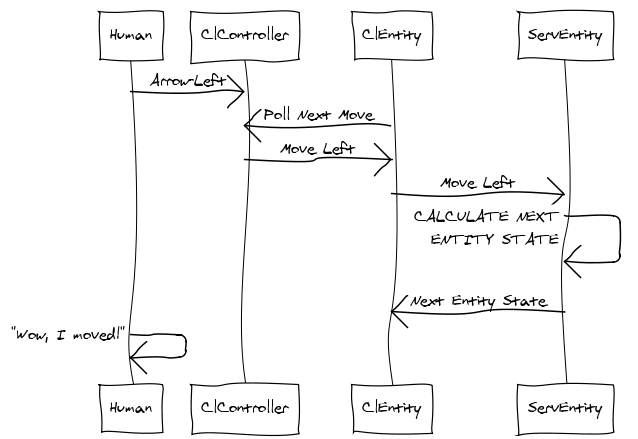
\includegraphics[width=0.50\textwidth]{images/netwerkfreq.png}
%	\caption{The client entity polls its next move from the controller}
%	\label{fig:netwerkfreq}
%\end{figure}
%
%\begin{figure}
%	\centering
%		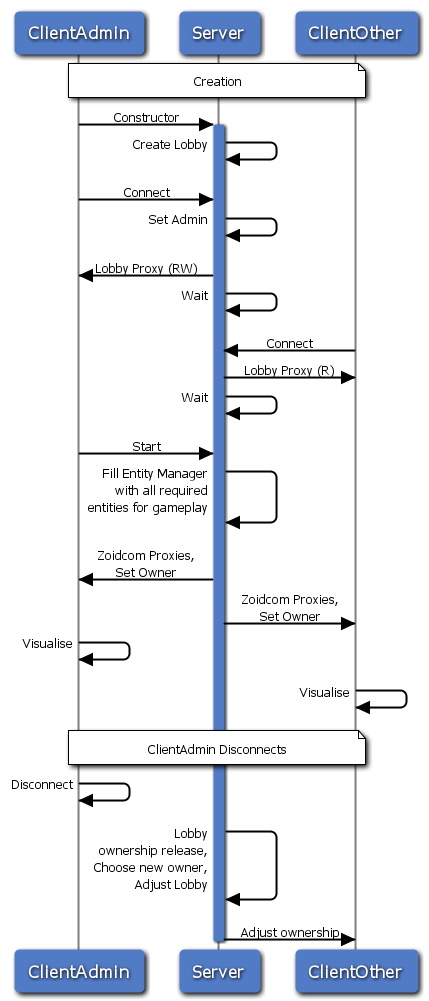
\includegraphics[width=0.50\textwidth]{images/zoidcom.png}
%	\caption{ZoidCom werking}
%	\label{fig:zoidcom}
%\end{figure}

De netwerkstructuur achter Hovercraft Universe is gebaseerd op het client-server model. De server is de instantie waar iedereen mee verbindt en deze maakt alle beslissingen in het spel. De server maakt deze beslissingen op basis van informatie die verkregen wordt via de clients. De clients verwerken de input van de gebruiker en sturen deze door naar de server. De server stuurt zijn beslissingen terug naar de clients die op hun beurt de wereld correct weergeven aan de gebruiker. Op deze manier wordt ervoor gezorgd dat clients geen game logic beslissingen kunnen maken.

Het client-server model wordt gebruikt voor zowel multiplayer als singleplayer. Hovercraft Universe biedt twee mogelijkheden om een multiplayer spel te starten. De eerste mogelijkheid is een dedicated server starten zonder grafische output. Clients kunnen verbinden met de dedicated server door het IP-adres van deze server in te geven. De tweede mogelijk is om een client samen met een server te draaien. De server zal gestart worden wanneer een client een multiplayer game cre\"eert. Andere clients zien geen verschil tussen een dedicated server of een gewone server. Een singleplayer spel bestaat ook uit een server en een client in \'e\'en instantie van het spel. De client zal met \emph{localhost} verbinden en zo een singleplayer spel kunnen spelen.

Het netwerk is gebaseerd op de ZoidCom netwerk library. Deze biedt de mogelijkheid voor replicatie van objecten en synchronisatie van de toestand van netwerk connecties via een high-level UDP protocol. Elke instantie in Hovercraft Universe is een object dat gerepliceerd wordt via het netwerk. Een voorbeeld hiervan is de hovercraft waarmee de speler racet. Dit object wordt aangemaakt op de server en deze laat dit weten aan de clients. De clients maken een \emph{proxy} object voor het hovercraft object. De server kan het hovercraft object aanpassen door de toestand ervan aan te passen. De netwerklaag zal controleren op updates en deze repliceren naar de proxy objecten bij de clients. De client die dit hovercraft object bestuurt, heeft de toestemming om events te sturen voor dit object die aangeven in welke richting de speler wilt bewegen. De netwerklaag zorgt dus voor het repliceren van objecten waardoor clients altijd de laatste toestand van deze objecten ontvangen.

Hovercraft Universe biedt ook de mogelijkheid voor communicatie tussen de spelers. Bij het starten van een gewone of dedicated server wordt er ook aparte een chat server opgestart. Clients verbinden met deze chat server en kunnen in de lobby en tijdens het spel via deze server met elkaar chatten. De chat server werkt net zoals de objecten in het spel met replicatie om de clients op de hoogte te houden van de laatste berichten.

\subsection{Modellen en user-data}
De \textbf{modellen} zijn gedefinieerd in het (niet open) bestandsformaat van 3DS Max. Deze worden ge\"exporteerd naar het DotScene XML-formaat met behulp van de OgreMax Scene Exporter\footnote{\url{http://www.ogremax.com/}}. DotScene\footnote{\url{http://www.ogre3d.org/wiki/index.php/DotScene}} is een gestandaardiseerd XML-formaat dat informatie bevat over het soort entiteit, de grootte van het model, de gebruikte materialen en meshfiles, etc. Tevens bevat dit DotScene bestand informatie specifiek voor gebruik in HovercraftUniverse (snelheid, gewicht, \ldots). Een voorbeeld van deze user-data is gegeven in Listing~\ref{lst:sceneuserdata}.

\lstset{language=XML,caption=UserData in DotScene,label=lst:sceneuserdata}
\begin{lstlisting}
<Hovercraft>
    <Name>USA Hovercraft</Name>
    <Description>Fast and responsive, rather light.
        </Description>
    <OgreEntity>USAHovercraft</OgreEntity>
    <ProcessInterval>0.016</ProcessInterval>
    <Speed>100</Speed>
    <Mass>50</Mass>
    <Acceleration>10</Acceleration>
    <Steering>100</Steering>
</Hovercraft>
\end{lstlisting}

Voor de \textbf{mappen} (tracks) wordt er \'e\'en groot DotScene wereld gegenereerd waarin alle relevante nodes zijn gedefinieerd: planeten, checkpoints, statische objecten, startposities, etc. Een voorbeeld van een dergelijke node is te zien in Listing~\ref{lst:jumpnode}

\lstset{language=XML,caption=E\'en van de nodes in de DotScene van een wereld.,label=lst:jumpnode}
\begin{lstlisting}
<node name="Jump01">
    <position x="-148.891" y="21.0134" z="-20.245" />
    <scale x="1" y="1" z="1" />
    <rotation qx="0.13454" qy="0.990908" 
        qz="-5.34715e-008" qw="-7.48115e-008" />
    <entity name="Jump01" castShadows="true" 
           receiveShadows="true" meshFile="Jump01.mesh">
        <userData>
            <![CDATA[<OgreEntity><GameEntity>Jump01_ent
                </GameEntity></OgreEntity>]]>
        </userData>
        <subentities>
            <subentity index="0" materialName="Jump02" />
        </subentities>
    </entity>
</node>
\end{lstlisting}

Door middel van scene loaders kunnen objecten gepositioneerd en getransformeerd worden om volledige sc\`{e}nes te  cre\"{e}ren. Het spel laat toe volledig uitgebreid en aangepast te worden door data files aan te passen zonder nood aan hercompilatie. Dit data-driven model beperkt zich niet alleen tot het toevoegen van werelden, maar ook tot het invoegen van nieuwe hovercrafts en characters. Tevens kan de kwaliteit van de werelden dynamisch worden aangepast door schaduws, lichten en materials aan en uit te zetten om zo ook oudere systemen te ondersteunen.

\subsection{Visualisatie en Ogre}

Ook worden hier een aantal visuele effecten aan toegevoegd. Ogre Particle Systems worden gebruikt om rook, vonken, etc. weer te geven. Er is tevens een tekst-overlay voor de nicknames voorzien zodat de spelers elkaar kunnen herkennen tijdens het spel. Aangezien deze effecten enkel client-side gebeuren bij het tekenen van de entiteiten, heeft dit geen invloed op de performantie van de netwerkcomponenten.

Schaduws en lichteffecten kunnen zoals voordien dynamisch aangepast worden. SkyX wordt gebruikt om dag- en nacht cycli te renderen en om wolken en sterrenhemels te tonen. Omdat het spel zich in de ruimte afspeelt wordt er enkel gerenderd tussen 22.00 en 5.00 uur. Beperkend aan SkyX is echter dat in de huidige vorm enkel hemels worden gerenderd en dus geen hele universe vol sterren. OgreMax\footnote{\url{http://www.ogremax.com/}} wordt gebruikt om modellen te exporteren vanuit 3DS Max en te importeren in Ogre.

Hovercraft Universe ondersteunt vier verschillende camera's: een third-person view waarbij de hovercraft zelf zichtbaar en waarbij een groot deel van de wereld wordt getoond. First-person view geeft een beter snelheidsgevoel en verhoogt het inlevingsvermogen van de speler. Vervolgens is er een rear-view camera en een free-roaming camera om de omgeving te verkennen.

Material mapping wordt gedetailleerd uitgevoerd door middel van UVW-unwrapping. Niet alleen is dit erg flexibel om gecontroleerd materials te geven aan modellen, ook laat dit single-pass GPU pixel shading toe en vergemakkelijkt dit het proces voor LoD. 

Het gebruik van pixel shaders wordt extensief aangewend om alpha splatting te verwezenlijken en dus de overgang tussen texture tiles vloeiend te laten overkomen. 

\subsection{Physics}

Alle acties op de hovercrafts en interacties met de omgeving gebeuren door middel van fysische krachten. Dit gebeurt volledig op de server, die een Havok-thread draait. De input van de clients, zowel menselijke spelers als AI, wordt vertaald in een kracht op de hovercraft. Havok berekent vervolgens alle totale krachten en daaruit volgende versnellingen en snelheden. Hieruit zal de nieuwe positie van alle entiteiten bepaald worden. Deze posities worden dan doorgestuurd naar alle clients zodat zij de wijzigingen kunnen zien. Bovendien zorgt Havok ook voor de collision detection zodat verschillende entiteiten niet tegelijk op dezelfde plaats kunnen bestaan. Collision detection gebeurt zowel tussen hovercrafts en stilstaande objecten als tussen hovercrafts onderling. Bij deze botsingen worden er bovendien vonkjes weergegeven door middel van particle effects.

De zwaartekracht op de verschillende planeten is afgeleid van het \texttt{PlanetGravity} voorbeeld van Havok. Concreet wordt er rond elke planeet een \textit{phantom} geplaatst. Wanneer een object binnen deze phantom komt, wordt er een kracht uitgeoefend waardoor de objecten aangetrokken worden door de planeet. Deze kracht kan per planeet verschillen zodat elke planeet een eigen zwaartekrachtsterkte heeft.

Op elke hovercraft-entiteit wordt nog een extra actie gedefini\"eerd om het object te laten zweven. Dit is een kracht die in tegengestelde richting ten opzichte van de zwaartekracht werkt. Afhankelijk van de hoogte verandert de grootte van de kracht. Dicht bij het planeetoppervlak zal er een sterke tegengestelde kracht gebruikt worden. Hoe verder van de planeet, hoe zwakker de kracht wordt. Vanaf een bepaalde hoogte valt de kracht weg, zodat de hovercraft terug naar beneden begint te vallen. Op deze manier krijgen we een lichte oscillatie van de hoveringhoogte.

De jumps tussen de verschillende planeten werken op dezelfde wijze. Wanneer een hovercraft in de phantom van zo'n jump komt, wordt een extra versnelling op de hovercraft uitgeoefend in de richting van de boost. Hierdoor kan het zwaartekrachtveld van de planeet overwonnen worden zodat het mogelijk is om naar de volgende planeet te springen.

\subsection{Grafische user interface}
De onderdelen van de GUI zijn ge\"implementeerd in ActionScript\footnote{\url{http://www.adobe.com/devnet/actionscript/}}, en worden met behulp van Hikari gevisualiseerd in Ogre. Hikari is een library die Flash (SWF) bestanden kan inlezen, en voor de binding tussen Flash en C++ zorgt. Hikari is aangepast en uitgebreid, oa. met de functionaliteit om overlays uit te schakelen.

De \texttt{BasicOverlay} klasse bevat alle basisfunctionaliteit en stelt een enkel Flash-bestand voor. Deze kan een bepaalde positie en dimensies innemen.

De HUD van het spel is geconfigureerd aan de hand van een XML-bestand. Gebruikers kunnen hun eigen HUD zo aanpassen, instellen en eventueel andere HUD-elementen gebruiken. Listing~\ref{lst:hudxml} toont een voorbeeld van de configuratie van een HUD-element.

\lstset{language=XML,caption=HUD configuratie van de LapTimer,label=lst:hudxml}
\begin{lstlisting}
<element type="timer" file="lapTimer.swf">
    <size>
       <min width="174" height="40" />
           <max width="520" height="120" />
    </size>
    <position>
        <relative val="TopRight" />
    </position>
</element>
\end{lstlisting}

\subsection{Geluid}
De FMOD library en tools zijn gebruikt voor het geluid en de muziek. De muziek is onderverdeeld Deze queues worden georganiseerd in een stack. De muziek en geluidseffecten worden door de FMOD Designer gecompileerd in \'e\'en enkel .fsb bestand.

Om toe te laten dat entiteiten in de wereld geluid produceren is \texttt{Moveable}- \texttt{3DEmitter} gemaakt. Deze is een wrapper voor de FMOD functionaliteit, en bepaalt het geluid voor een entiteit in de wereld aan de hand van de positie, snelheid, orientatie. In onze architectuur zorgen de \texttt{EntityRepresentation}s voor de specifieke implementatie van het 3D geluid.

\subsection{Besturing}
De centrale klasse voor de besturing is de \texttt{KeyManager}. In deze klasse kunnen alle nodige acties geregistreerd worden door middel van een uniek ID, bijvoorbeeld in een enumeratie. Aan elk van deze acties kunnen \'e\'en of meerdere knoppen gebonden worden. Telkens wanneer de \texttt{HovercraftPlayerController} een key event binnenkrijgt, zal er bij de key manager nagegaan worden welke actie er overeenkomt met deze toets. Op deze manier is het mogelijk om de spelbesturing gemakkelijk te wijzigen zonder dat de controller aangepast moet worden. Bovendien kunnen er meerdere toetsen voor dezelfde actie gebruikt worden.

In de \texttt{KeyManager} staat ook nog een mapping tussen alle toetsen die OIS ondersteunt en hun bijhorende string-representatie. Zo kunnen de controls ingelezen of weggeschreven worden naar een configuratiebestand. Standaard is dit bestand te vinden in de data\textbackslash controls map, maar wanneer dit bestand ontbreekt zal er automatisch een nieuw aangemaakt worden met de default controls. In dit configuratiebestand staan alle geregistreerde acties per categorie. Voor elke actie kunnen \'e\'en of meerdere toetsen opgegeven worden, gescheiden door een komma. Wanneer een actie ontbreekt, zal de standaardtoets voor deze actie gebruikt worden.

\subsection{Scripting en AI}
Voor de bots is een AI voorzien, die ``menselijk'' stuurgedrag nabootst. De algoritmen van deze AI zijn gebaseerd op de autonome stuursimulaties van Craig Reynolds \cite{reynolds:1999}. De huidige AI is in staat om een voorgedefinieerd pad te volgen binnen een bepaalde marge (``Path Following''). Een pad wordt voorgesteld als een \emph{multiline}: een lijst van punten in de wereld, telkens geassocieerd met een straal (\texttt{radius}). De straal op punt $x_i$ stelt de \emph{breedte} van het pad voor tussen punt $x_i$ e, $x_{i+1}$. Deze paden worden opgeslagen in aparte bestanden. Dit betekent dat de level designers per map een ideaal pad (of meerdere paden) voor de AI kunnen aanmaken. 

De AI is geprogrammeerd in Lua \cite{lerusalimschy:2006}, om aanpassing van de AI-algoritmen mogelijk te maken zonder dat het spel hiervoor gehercompileerd moet worden. Voor de binding tussen Lua en C++ wordt Luabind gebruikt. De \texttt{ScriptWrapper} klasse abstraheert deze scripts en laat de programmeurs toe om met de scripts te werken, zonder Lua-specifieke constructies te moeten gebruiken.

\emph{Collision avoidance} voor de AI is ook ge\"implementeerd met behulp van Havok physics. Er zijn twee implementaties beschikbaar voor de \texttt{EntityCollision} interface. Het eenvoudige model (zie Figuur~\ref{fig:simplecollisionavoidance}) plaatst een kubus op een bepaalde afstand van het voertuig om objecten te detecteren. Dit model gebruikt zeer weinig resources, maar is ook niet zo krachtig. Het geavanceerde model gebruikt een 3D-lichaam dat zich uitstrekt van het voertuig tot de gewenste afstand voor de figuur (zie Figuur~\ref{fig:advancedcollisionavoidance}). Deze manier van werken heeft een kleine meerkost in resources in vergelijking met het eenvoudige model.

Aangezien deze methodes afhankelijk zijn van de physics, draaien ze op de server. Als een object wordt gedetecteerd, wordt dit door middel van een event doorgegeven aan een callback functie in de entiteit. Dit wordt vertaald naar een boolean in de entiteit, die door het netwerk wordt gerepliceerd op de client. Client-side maakt de AI dan een beslissing om het obstakel te ontwijken.

\begin{figure}%
\begin{center}
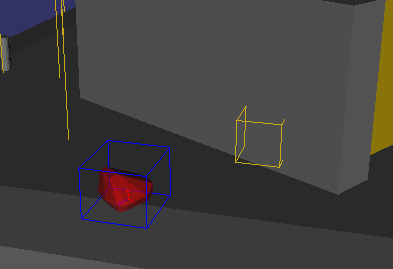
\includegraphics[width=0.6 \columnwidth]{images/collision_prevention_simple.jpg}%
\end{center}
\caption{Het eenvoudige collision avoidance model}%
\label{fig:simplecollisionavoidance}%
\end{figure}

\begin{figure}%
\begin{center}
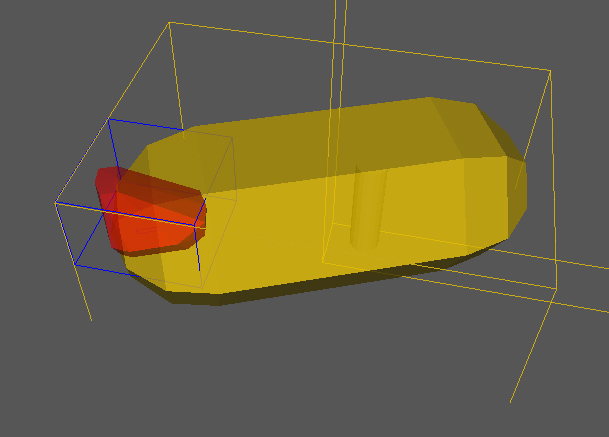
\includegraphics[width=0.8 \columnwidth]{images/collision_prevention_advanced.jpg}%
\end{center}
\caption{Het geavanceerde collision avoidance model}%
\label{fig:advancedcollisionavoidance}%
\end{figure}

\subsection{Game Logic}

Bij het starten van een multiplayer spel komen de spelers eerst in een lobby. De lobby bevat de logica om een spel te starten met een aantal speler. De eerste speler, die met de lobby verbindt, wordt automatisch administrator. Deze speler kan de verschillende instellingen van de lobby aanpassen, v.b. het aantal spelers en de map. De administrator kan ook beslissen wanneer het spel start. De lobby zal op dat moment de objecten van de gekozen map en de objecten voor alle spelers aanmaken. Als de administrator het spel verlaat, kiest de lobby een nieuwe administrator die de instellingen kan aanpassen.

De lobby zal bij het starten van de map ook een RaceState object maken. Dit object bevat alle logica die nodig is tijdens het spel en zal ook eventuele bots aanmaken. De RaceState start in de \emph{INTRO} staat en zal een countdown starten zodat de spelers tesamen vertrekken. Tijdens de race gaat de RaceState naar de \emph{RACING} staat en zal bij elke checkpoint de nieuwe posities berekenen voor de spelers. Het tijdstip van de checkpoint wordt voor elke speler bijgehouden en doorgestuurd naar alle spelers zodat deze op de hoogte worden gehouden van de status van de andere spelers.

\subsection{Level of Detail}
\subsubsection{Netwerk}

De snelheid waarin updates worden gebroadcast naar andere avatars wordt dynamisch aangepast door middel van prioriteiten. Zoidcom bevat functionaliteit om bepaalde objecten relevanter of minder relevant te maken zodat deze sneller of minder snel worden ge\"updatet en worden doorgestuurd naar de clients. Deze relevantie wordt in Hovercraft Universe enerzijds bepaald door de afstand in wereldco\"{o}rdinaten, maar ook door de planeten waar we op zitten. Updates van andere objecten worden sneller ontvangen als deze zich op dezelfde planeet vinden dan wanneer ze zich op een andere planeet bevinden. 

Om de hoeveelheid updates te verminderen  wordt er gebruik gemaakt van dead reckoning. Concreet betekent dit dat er een positie en een richting wordt doorgestuurd naar de clients en dat deze zelf berekenen waar de entiteiten zich de volgende frames zullen bevinden tot er een nieuwe update binnenkomt van de server en de correcte nieuwe positie en richting wordt ingesteld. Het berekende pad wordt dan ge\"{i}nterpoleerd naar de ge\"{u}pdatete posities. Door dit toe te passen kan de benodigde frequentie van de updates sterk verlaagd worden. Een eventuele discrepantie met betrekking tot bijvoorbeeld collision detection wordt opgelost doordat de hele collision engine server-based gebeurt en deze inherent een consistente staat van de wereld bevat. Bij bijvoorbeeld botsingen worden dan events gegenereerd die onmiddelijk de staat op de client aanpassen zodat kritische acties meteen bij alle relevante clients zichtbaar worden.


\subsubsection{Rendering}

Ogre bevat reeds een standaard aantal algoritmes voor LoD. Dit wordt zoals reeds vermeld in de hand gewerkt door een slim gebruik van textures. De mate waarin LoD wordt toegepast kan dynamisch worden aangepast in configuratiebestanden.

\subsection{Misc.}

\subsubsection{Configuratiebestanden}
Configuratiebestanden zijn beschikbaar voor de server en client, in INI formaat (zie Listing~\ref{lst:inifileformat}). Dit laat gebruikers toe om hun nickname, gekozen voertuig, enz. te kiezen en op te slaan. Een aantal server-specifieke instellingen worden ook ondersteund (aantal spelers, AI-script, sterkte van de zwaartekracht, \ldots). Het spel kan deze bestanden ook opslaan met de huidige instellingen.

\lstset{caption=Het INI bestandsformaat,label=lst:inifileformat}
\begin{lstlisting}
[section name]
keyname=value
#comment
keyname = value, value , value #comment
\end{lstlisting}

\section{Rolverdeling en verantwoordelijkheden}
\begin{description}
	\item[Kristof Overdulve] Algemene client rendering architectuur, Ogre visualisatie en animatie, 2D artist, 3D modellering
	\item[Pieter-Jan Pintens] Havok Physics, 3D modellering, Ogre visualisatie en animatie
	\item[Dirk Delahaye] Scripting, AI, visuele effecten, configuratiebestanden
	\item[Tobias Van Bladel] Input, controls, physics
	\item[Nick De Frangh] Grafische user interface, Geluid
	\item[Olivier Berghmans] Algemene server architectuur, netwerk
\end{description}

\bibliographystyle{plain}
\bibliography{references}

\end{document}
